\documentclass[12pt]{article}
\usepackage[a4paper]{geometry}               

\usepackage[parfill]{parskip}    % Activate to begin paragraphs with an empty line rather than an indent
\usepackage{graphicx}
\usepackage{amssymb}
\usepackage{yfonts}
\usepackage[cal=dutchcal]{mathalfa}
%\usepackage[mathcal]{euscript}
\usepackage{amsmath}
%

\usepackage[skip=15pt,font=footnotesize,labelfont=bf]{caption}
%

\title{Technical Note: Sharma-Mittal Generalized Entropy and 'Code Jar' Mastermind}
\author{Matthias Hofer$^*$, Jonathan D. Nelson\footnote{Max Planck Institute for Human Development, Berlin}}
%\date{}                                           % Activate to display a given date or no date

\begin{document}
\maketitle

{\footnotesize \textbf{Abstract.} $\quad$ We consider a variation of the well-known game of Mastermind to explore entropy-based approaches to the design of effective playing strategies. Our main goal is to conduct computer simulations to explore different entropy measures from a unified mathematical formalism, called the Sharma-Mittal generalized entropy framework. Ultimately, our goal is to translate potential theoretical findings to the domain of human psychology to investigate human intuitions about the informativeness of different queries when playing Mastermind.}

\tableofcontents

\pagebreak
\section{The Mastermind Game}
\subsection{Standard version}
In the original game, the \textit{code maker} composes a hidden code $c_h$ of fixed length $\mathcal{l}$ using a combination of pegs (or marbles) of $\mathcal{n}$ different colors (repetitions are allowed). Here we will use the set of integers $\mathcal{A} = \{1, ..., \mathcal{n}\}$ to represent the different-colored pegs. Call $\mathcal{E} = \{\mathcal{A}\}^\mathcal{l}$ the set of all possible \textit{combinations} of symbols from $\mathcal{A}$ of length $\mathcal{l}$, including the hidden code $c_h$. 

Each round the \textit{code breaker} takes a guess at the code and receives feedback about the number of pegs in the right position $b$ (black token) and, additionally, the number of pegs that are of the right color but at the wrong place $w$ (white token). Let $c_{i}$ denote the code breaker's guess and $r_i=(b_i,w_i)$ the corresponding feedback, respectively, at round $i$. 

Using the feedback provided after each guess, the code breaker's goal is to guess the hidden code $c_h$ in as few rounds as possible. The game ends when $c_i = c_h$, which is equivalent to $r_i=(\mathcal{l},0)$. In formal notation, a standard Mastermind game can be represented by the tuple

\[\mathcal{G}_{standard}=\Big(\mathcal{A}, \mathcal{l}\Big),\]

with $\mathcal{n} = |\mathcal{A}|$ and $\mathcal{E} = \{\mathcal{A}\}^\mathcal{l}$. Note the constraints on receiving feedback: 
\begin{itemize}
\item $b$ + $w \leq \mathcal{l}$
\item  if $b = \mathcal{l}-1$, then $w = 0$
\end{itemize}
Call $\mathcal{R_l}$ the set of all possible combinations $r=(b,w)$ for feedback. For $\mathcal{l} = 3$, for instance:

\begin{align*}
\begin{split}
\mathcal{R_3} = \{ &(0,0), \\
			 &(0,1), (0,2), (0,3), \\
			 &(1,1), (1,2), \\
			 &(2,0), \\
			 &(3,0) \}
\end{split}
\end{align*}

Or, more generally, $\mathcal{R_l} = \{ (0,0), (0,1), ..., (0,\mathcal{l}), (1,1), ..., (1,\mathcal{l}-1), ...,  (\mathcal{l}-1,0), (\mathcal{l},0) \}$, where $|\mathcal{R_l}| = |\mathcal{R_{l-1}}| + \mathcal{l}$ with $|\mathcal{R_1}| = 3$.


\subsection{Code jar version}

Here we consider a variation of the standard game that involves introducing a \textit{code jar} from which the hidden code is sampled (with replacement) by the code maker. A code jar $J$ is an arbitrary set of pegs of different colors that (implicitly) defines a probability distribution $\mathcal{P}_J$ over the set of different-colored pegs $\mathcal{A}$. The code jar version is defined by the triple

\[\mathcal{G}_{code jar}=\Big(\mathcal{A}, \mathcal{l}, {J}\Big),\]

with $\mathcal{n} = |\mathcal{A}|$, $\mathcal{E} = \{\mathcal{A}\}^\mathcal{l}$ and $\mathcal{P}_J(\mathcal{A})$ directly following from the quantities specified in $\mathcal{G}_{code jar}$. Rules for constraints on $\mathcal{R_l}$ are precisely as in the standard version (see ablove).

Note that the standard game can be seen as a special case of the code jar version when the code jar defines a uniform distribution over all possible symbols (pegs). This can be achieved by, for instance, setting ${J}=\{\{1\},\{2\},...\{\mathcal{n}\}\}$, where the code car contains exactly one peg for each of the $\mathcal{n}$ colors.

\section{Important concepts}

Mastermind is a dynamic constraint optimization problem. It is dynamic because the constraints determining the solution space are not known a priori and depend on the course of the game (i.e., the combinations played and the hidden code). One key notion is feasibility. The \textit{feasible set} can be determined deductively by considering which combinations are consistent with the guesses made so far and the received feedback. We denote the feasible set after guess $i$ with $\mathcal{F_i}$. Feasibility is a transient property. Initially, all combinations in $\mathcal{E}$ (={}$\mathcal{F_0}$) are feasible. A combination looses its feasibility when it is inconsistent with any of the guesses made by the code breaker. The notions of consistency and feasibility (see below) hold for both the standard as well as the code jar version of the game.

\subsection{Consistency}

Consistency is a non-symmetric, reflexive function of two combinations $c_q$ and $c_r$. We say that combination $c_q$ is consistent with $c_r$, when h($c_q$, $c_r$) = h($c_r$, $c_h$), where h($c_q$, $c_r$) refers to the feedback when playing combination $c_q$, and when $c_r$ is the hidden code. I.e., $c_q$ is consistent with $c_r$ iff $c_q$ generates the same feedback under  $c_r$ as hidden code than  $c_q$ generates under $c_h$. If a combination is consistent with all past guesses $c_i$, it is logically consistent to assume that it is the hidden combination. 

\subsection{Feasibility and the feasible set}

All combinations that are consistent after guess $i$ are part of the feasible set $\mathcal{F_i}$. 
The feasible set will shrink after each round unless no combination $c_i$ is repeatedly used as a guess (in which case the feasible set stays the same).


\section{Determining the usefulness of a combination}

A generic playing strategy for Mastermind consists of procedures for (i) identifying the set of feasible combinations $\mathcal{F_i}$ (with $\mathcal{F_0}=\mathcal{E}$), where prior feedback is used to determine which combinations are still viable and which not; and (ii) picking the combination $c_{i+1}$ for the next guess. While for the standard version, the usefulness of a combination depends on how many combinations it is expected to exclude in the next step, this does not necessarily hold for the probabilistic, code jar version of the game. 

\subsection{Graphical intuition}

Since not all combinations in $\mathcal{E}$ are necessarily equally likely, we have to use a different utility function to measure how much we prefer one feasible set over another. For example, ending up with a set $\mathcal{F^a}$ with $P(\mathcal{F^a})=\{0.6, 0.1, 0.1, 0.1, 0.1\}$ is (arguably) better than ending up with $\mathcal{F^b}$ with $P(\mathcal{F^b})=\{0.2, 0.2, 0.2, 0.2, 0.2\}$, if we had to take a guess at the hidden code. We will use the notion of entropy to quantify this difference, i.e., to measure the uncertainty of a probability distribution. Building on this, our algorithm (introduced below) chooses the combination that provides the highest expected reduction in entropy. A graphical intuition on how to compute the usefulness of a combination $c$ is provided in Figure \ref{fig:u} and a formal description follows in the next section. 

\begin{figure}[h]
\centering
%\captionsetup{format=hang}
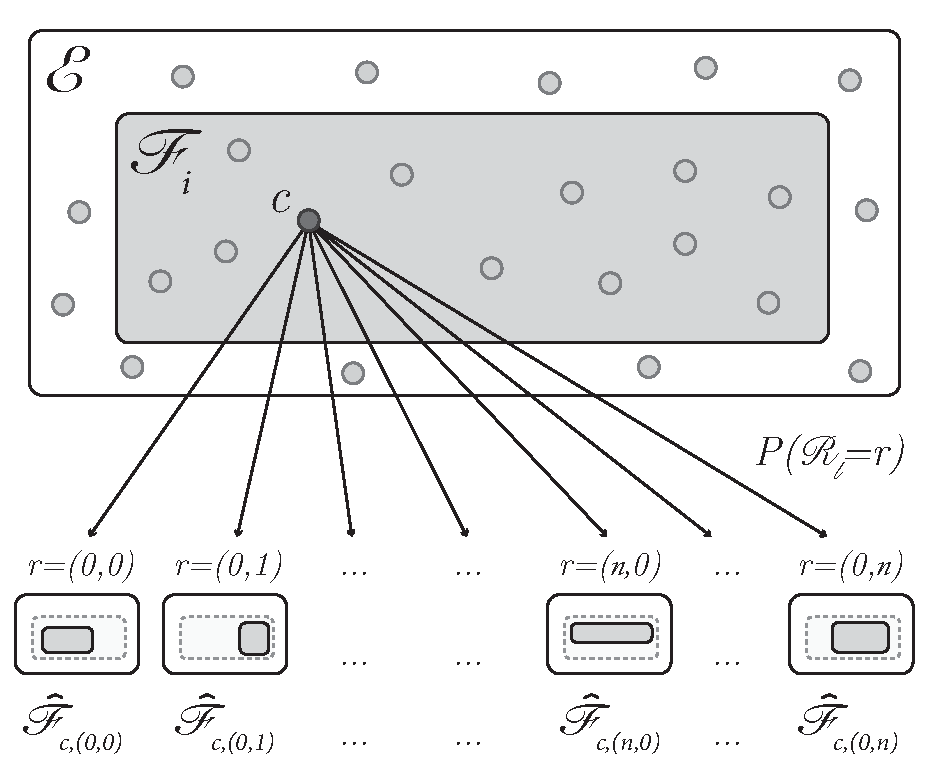
\includegraphics[width=.65\textwidth]{graphical-intuition}
\caption[Graphical Intuition]{Graphical intuition for computing the usefulness of a query. After guess $i$, the current feasible set $\mathcal{F}_i$ is a subset of the set $\mathcal{E}$, containing all possible combinations. We can evaluate the usefulness of any combination $c$ (not necessarily only combinations in $\mathcal{F}_i$) by considering all possible combinations of feedback $r$ when playing $c$ and their respective probabilities $P(\mathcal{R_l}=r)$. We can also compute the ensuing feasible sets $P(\mathcal{\hat{F}}_{c,r})$, the possible worlds we could end up in after receiving feedback $r$ when playing combination $c$. The usefulness of query $c$ is then defined as the probability-weighted sum of $H(\mathcal{F}_{c,r})$, where $H$ measures the entropy of the set.}
\label{fig:u}
\end{figure}


\subsection{Formal treatment}

Let us denote the expected utility (or usefulness) of playing combination $c$ in the next round with $eu(c)$. The generic formula for computing $eu(c)$ is


\begin{equation} 
eu(c) = \sum_r^{\mathcal{R_l}}  P(\mathcal{R_l}=r) \cdot H^{SM_{r,t}} \Big ( P(\mathcal{\hat{F}}_{c,r}) \Big ),
\label{eq:u}
\end{equation} 


that is, for each possible feedback r, the product of the probability of receiving feedback r, $P(\mathcal{R_l}=r)$, and the entropy associated with the ensuing feasible set $\mathcal{\hat{F}}_{c,r}$ when playing combination $c$ and receiving feedback $r$. We will look at each of these quantities and how to compute them below.

\subsubsection{Probability of feedback}

The general idea behind the formula above is to consider all possible outcomes (feedback) when playing combination $c$ and to ask how much we 'like' receiving a particular feedback. Let us first consider how to compute the probability of different feedback outcomes. 

When taking into account that same combinations might already have been eliminated from the feasible set, the potential feedback will be a subset of $\mathcal{R_l}$. To compute $P(\mathcal{R_l}=r)$, the probability of receiving some feedback $r$ from set $\mathcal{R_l}$, we simply look at all the combinations in $\mathcal{F}_i$ that would lead to feedback $r$ when they were the hidden code. For some combination $c$,

\[ P(\mathcal{R_l}=r) = \frac{\sum_{c_j}^{\mathcal{F}} P(c_j) \cdot \gamma_r(c, c_j)}{\sum_{c_i}^{\mathcal{F}} \sum_{c_j}^{\mathcal{F}} P(c_j) \cdot \gamma_r(c_i, c_j)}, \]


where $\gamma_r(c, c_j) = 1$ if $h(c, c_j)=r$ and $0$ otherwise to ensure we only include combinations that are feasible with $c$ under $r$. The probability of any combination of pegs or \underline{m}arbles $c=m_1m_2...m_\mathcal{l}$ can be computed as

\label{eq:p}
\begin{equation} 
P(c=m_1m_2...m_\mathcal{l}) = \mathcal{P}_J(\mathcal{A}=m_1) \cdot \mathcal{P}_J(\mathcal{A}=m_2) \cdot ... \cdot \mathcal{P}_J(\mathcal{A}=m_\mathcal{l})
\end{equation} 

for the code jar version, and $P(c=m_1m_2...m_\mathcal{l}) = (\frac{1}{\mathcal{n}})^{l}$ for the standard version.



\subsubsection{Determining hypothetical feasible sets}

The other term of Equation \ref{eq:u} is $H^{SM_{r,t}} ( P(\mathcal{\hat{F}}_{c,r}) )$, which requires us to compute hypothtical feasible sets ${\hat{\mathcal{F}}}_{c,r}$ (also see Figure \ref{fig:u}). Given the current feasible set $\mathcal{F}_i$, a combination $c_i$ we want to evaluate, and hypothetical feedback $r$, we simply need to exclude all combinations $c_j \in \mathcal{F}_i$ for which $h(c_j, c_i) \neq r$; that is, all combinations $c_j$ that are not consistent with feedback $r$.

\subsubsection{Sharma-Mittal generalized entropy}

Lastly, in order to measure how much we 'like' one such hypothetical set, i.e., to assign a utility to a feasible set $\mathcal{F}$, we use the notion of entropy. We use the generic Sharma-Mittal entropy framework to compute the entropy of a probability distribution defined over set $\mathcal{F}$, $P_{\mathcal{F}}(c)$. For each combination $c \in \mathcal{F}$

\begin{equation*}
P_{\mathcal{F}}(c) = \frac{P(c)}{\sum_{c_j}^{\mathcal{F}} P(c_j)},
\end{equation*}

where the nominator $P(c)$ is computed according to Equation \ref{eq:p} and the denominator is a normalization term. The Sharma-Mittal entropy of set $\mathcal{F}$ can then be computed as 

\begin{equation*}
H^{SM_{(r,t)}}\big( {\mathcal{F}} \big)=\frac{1}{t-1}\Bigg[ 1-\bigg(\sum_{c}^{\mathcal{F}} P_{\mathcal{F}}(c)^r \bigg)^{\frac{t-1}{r-1}} \Bigg],
\end{equation*}

where $0 < r,t < \infty$.

%We first compute the (current) feasible set $\mathcal{F}$. We then compute the probability of receiving different feedback $r$ when playing combination $c_i$. $R_{c_i}$ is a random variable that takes as values different possible combinations of $b$ and $w$:
%
%\[R_{c_i}=\{(1,0), (2,0), ..., (\mathcal{n},0),(1,1),(2,1), ...(\mathcal{n}-2,1),... (0,\mathcal{n})\} \]
%
%The probability of receiving feedback $r$ when playing combination $c_i$ can then be computed in the following way: 
%
%\[ P(R_{c}=r)=\frac{\sum_{c_j}^{\mathcal{F}} P(c_j) \cdot \gamma_r(c_j, c) }{\sum_{c_i}^{\mathcal{F}} \sum_{c_j}^{\mathcal{F}} P(c_j) \cdot \gamma_r(c_j, c_i)},\]
%
%where $\gamma_r(c_i, c_j) = 1$ if $h(c_i, c_j)=r$ and $0$ otherwise. The expected usefulness $eu$ of playing combination $c_i$ can then be defined in the following way: 
%
%\[ eu(c) = \sum_r  P(R_{c}=r) \cdot \epsilon (r,c), \]
%
%with $\epsilon(c,r) = ent_{SM_{r,t}} \Big (P(\mathcal{F}_{c,r}) \Big )$
%For each (feasible) combination, we can consider all possible types of feedback we can get




%\section{SMENT: An entropy-based strategy for code jar Mastermind}




%A generic playing strategy consists of: (i) procedures for identifying in each round the set of feasible combinations, where prior feedback is used to determine which combinations are still feasible and which not; and (ii) procedures for picking the combinations that best serve the goal of reducing the number of feasible solutions as much as possible. 
%In our modified version of the game, the code is sampled with replacement from a code jar that contains an arbitrary number of pegs of each color. Each color is thus chosen with probability proportional to the number of pegs of that color in the code jar. This entails that the probabilities of different candidate solutions in the feasible might differ. Whereas in the standard version each combination is equally likely, a non-uniform distribution over colors in the code jar will lead to some combinations being more probable than others. To illustrate how this might impact the design of effective playing strategies, consider how an algorithm playing the game might choose between two alternative guesses, each resulting in sets of five feasible combinations, but where the probabilities of set one and set two are [0.6, 0.1, 0.1, 0.1, 0.1] and [0.47, 0.47, 0.02, 0.02, 0.02], respectively. Which set would you rather end up with? 
%In order to quantify our uncertainty about the true code with respect to the remaining members in the feasible set, we use the notion of entropy. Previous approaches to devising efficient algorithms to solve the Mastermind problem used the well-known Shannon entropy measure [1]. 





\end{document}  